\documentclass[journal]{IEEEtran}
\usepackage[spanish]{babel}
\usepackage[utf8]{inputenc}
\usepackage{enumerate}
\usepackage{graphicx}
\usepackage{booktabs}
\usepackage{physics}

\hyphenation{op-tical net-works semi-conduc-tor}


\begin{document}
\title{Reporte de Práctica: Caída Libre }

\author{Licenciatura en Física	\\
Universidad Nacional Autónoma de México - Facultad de Ciencias\\
Profesor: José Alfredo Morales Pérez\\
Ayud. Lab.	Miranda García Ávila\\
Integrantes: Jeshua Roberto Estrada Ocampo,~\IEEEmembership{424003085}\\

            
\thanks{}% <-this % stops a space
\thanks{}% <-this % stops a space
\thanks{}}

\markboth{Laboratorio de Mecánica}%
{Shell \MakeLowercase{\textit{et al.}}: Bare Demo of IEEEtran.cls for Journals}

\maketitle

\begin{abstract}
En este reporte de laboratorio se presentó el estudio de la caída libre de objetos, un fenómeno fundamental en la mecánica clásica. El experimento se llevó a cabo para observar y analizar el comportamiento de un objeto en caída libre bajo la influencia de la gravedad, despreciando la resistencia del aire. Se midieron el tiempo de caída y la distancia recorrida por el objeto desde diferentes alturas. Los datos obtenidos se compararon con los valores teóricos previstos por las ecuaciones del movimiento uniformemente acelerado. Los resultados demostraron una concordancia significativa con la teoría, proporcionando una comprensión más profunda de los principios de la dinámica.
\end{abstract}

\begin{IEEEkeywords}
Caída libre, Gravedad, Movimiento uniformemente acelerado, aceleración
\end{IEEEkeywords}

\IEEEpeerreviewmaketitle

\section{INTRODUCCIÓN}
\subsection{Planteamiento}

\IEEEPARstart  {L}a caída libre es un fenómeno fundamental en la física clásica, siendo uno de los primeros experimentos que ilustran las leyes del movimiento formuladas por Sir Isaac Newton. Comprender la caída libre no solo es crucial para el entendimiento básico de la dinámica, sino que también tiene aplicaciones prácticas en campos tan variados como la ingeniería, la astronomía y la biología. La práctica de laboratorio se justifica por la necesidad de observar directamente el comportamiento de los objetos bajo la influencia exclusiva de la gravedad, excluyendo factores como la resistencia del aire. Esta observación empírica permite corroborar las predicciones teóricas y refinar nuestra comprensión de los principios físicos que gobiernan el movimiento de los cuerpos.\\

\subsubsection{Objetivos Generales}

 - Analizar el comportamiento de un objeto en caída libre para validar las predicciones teóricas del movimiento uniformemente acelerado debido a la gravedad.\\

\subsubsection{Objetivos particulares}
- Medir el tiempo de caída de un objeto desde diferentes alturas.\\
- Calcular la aceleración debida a la gravedad a partir de los datos experimentales.\\
- Evaluar las posibles fuentes de error y su impacto en los resultados obtenidos.\\

\subsubsection{Hipótesis}
Si un objeto cae en ausencia de resistencia del aire, su aceleración será constante e igual a la aceleración debida a la gravedad terrestre (aproximadamente \(9.8 \frac{m}{s^{2}}\)). Los tiempos de caída medidos experimentalmente permitirán calcular esta aceleración, y se espera que los valores obtenidos sean consistentes con el valor teórico de la gravedad.\\

\section{MARCO TEÓRICO}
La caída libre es el movimiento de un objeto bajo la influencia de la gravedad, sin la interferencia de otras fuerzas como la resistencia del aire. Este fenómeno ha sido ampliamente estudiado y es un concepto fundamental en la física clásica.
se define como el movimiento que experimentan los cuerpos cuando únicamente actúa sobre ellos la fuerza de la gravedad. En este caso, todos los cuerpos, independientemente de su masa, aceleran hacia la Tierra con una aceleración constante denominada aceleración de la gravedad, denotada como g.
la aceleración de la gravedad en la superficie de la Tierra es aproximadamente \(9.8 \frac{m}{s^{2}}\)) Este valor puede variar ligeramente dependiendo de la altitud y la latitud, pero para la mayoría de los cálculos g se considera constante. 

Las ecuaciones que describen el movimiento de un objeto en caída libre, suponiendo que parte del reposo, se derivan de las ecuaciones del movimiento uniformemente acelerado:
\begin{equation}\label{eq:1}
 y= y_0 + v_0t + \frac{1}{2}gt^2
\end{equation}

donde y y \(y_o\) son la posición inicial y final respectivamente, \(v_0\)es la velocidad inicial, t es el tiempo transcurrido durante el movimiento y g es la constante de gravedad.
También contamos con la ecuación de la velocidad dada por:

\begin{equation}\label{eq:2}
 v=v_o + tg
\end{equation}

En el contexto del experimento de caída libre, las ecuaciones anteriores se utilizan para calcular los parámetros del movimiento del objeto en caída libre. Mediante la medición del tiempo de caída y la altura desde la cual se deja caer el objeto, se pueden determinar las velocidades y la aceleración debida a la gravedad, permitiendo así una comparación con los valores teóricos.


\section{ MATERIALES}
\begin{itemize}
\item Flexómetro \item 2 pelotas de distinta masa  
\item Tripie \item Camara de celular \item software de análisis de video Tracker
\end{itemize}

\section{DESARROLLO EXPERIMENTAL}

Para realizar el experimento de caída libre de manera efectiva y obtener resultados precisos, es fundamental minimizar la influencia de factores externos como la resistencia del aire y asegurar condiciones controladas. Las condiciones ideales incluyen:

Eliminación de la Resistencia del Aire: Si bien en la práctica es difícil eliminar completamente la resistencia del aire, se pueden elegir objetos que minimicen su efecto, como esferas compactas y de alta densidad.\\
Ambiente sin Corrientes de Aire: Realizar el experimento en un lugar cerrado y sin corrientes de aire que puedan alterar la trayectoria de los objetos.\\
Superficie Plana y Nivelada: Asegurar que la superficie de la que se deja caer el objeto esté nivelada y a una altura conocida.\\
Medición Precisa del Tiempo: Utilizar dispositivos de cronometraje con alta precisión, como cronómetros digitales o grabaciones de video que permitan un análisis cuadro por cuadro.\\

Se coloca un flexómetro (cinta métrica) en una pared, fijándolo de manera segura para evitar desplazamientos durante el experimento. Esto nos proporcionó un marco de referencia vertical y permitió medir con precisión la altura desde la cual se dejaron caer los objetos.
La altura de referencia se estableció en 2 metros, y se marcó claramente en la pared.\\

Se eligieron 2 objetos para el experimento: pelotas de distintas masas.
Cada uno de estos objetos fue seleccionado para observar cómo la masa y la forma afectan la caída libre en condiciones prácticas.\\

Desde la altura de 2 metros, los alumnos dejaron caer los objetos uno a uno.
Para cada caída, se utilizó una cámara para grabar el movimiento. La grabación de video permitió un análisis detallado y preciso del tiempo de caída mediante el análisis cuadro por cuadro.
Este procedimiento se repitió para cada uno de los objetos.\\

A partir de las grabaciones de video, se midió el tiempo de caída de cada objeto desde el momento en que fue soltado hasta que alcanzó el suelo.
Se utilizó software de análisis de video para asegurar la precisión en la medición del tiempo.\\

Con los tiempos de caída medidos y la altura de 2 metros, se aplicaron las ecuaciones del movimiento uniformemente acelerado para calcular la aceleración debida a la gravedad.
La fórmula utilizada fue:

\begin{equation}\label{eq:2}
 g = \frac{2y}{t^2}
\end{equation}

\hfill 

\section{RESULTADOS}

\begin{figure}[h]
    \centering
    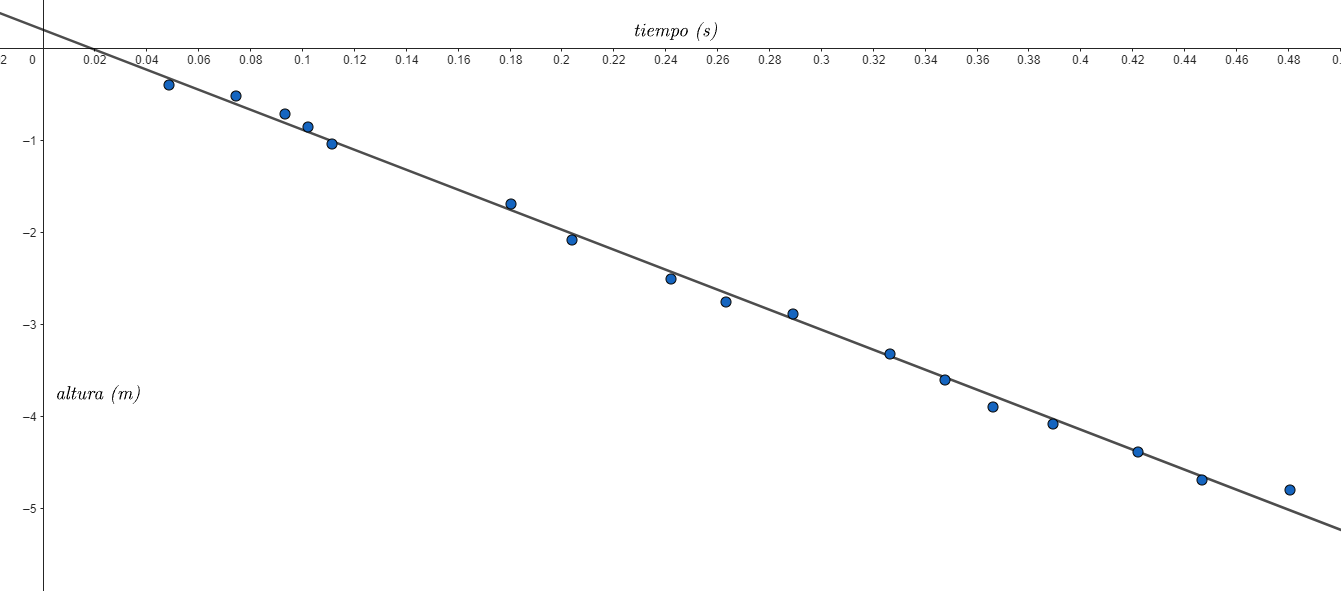
\includegraphics[width=1\linewidth]{vt1.png}
    \caption{Velocidad vs Tiempo (pelota 1)}
    \label{fig:enter-label}
\end{figure}

\begin{figure}[h]
    \centering
    
\includegraphics[width=1\linewidth]{image.png}
    \caption{Posición en $y$ vs Tiempo (pelota 1)}
    \label{fig:enter-label}
\end{figure}

\begin{figure}[h]
    \centering
    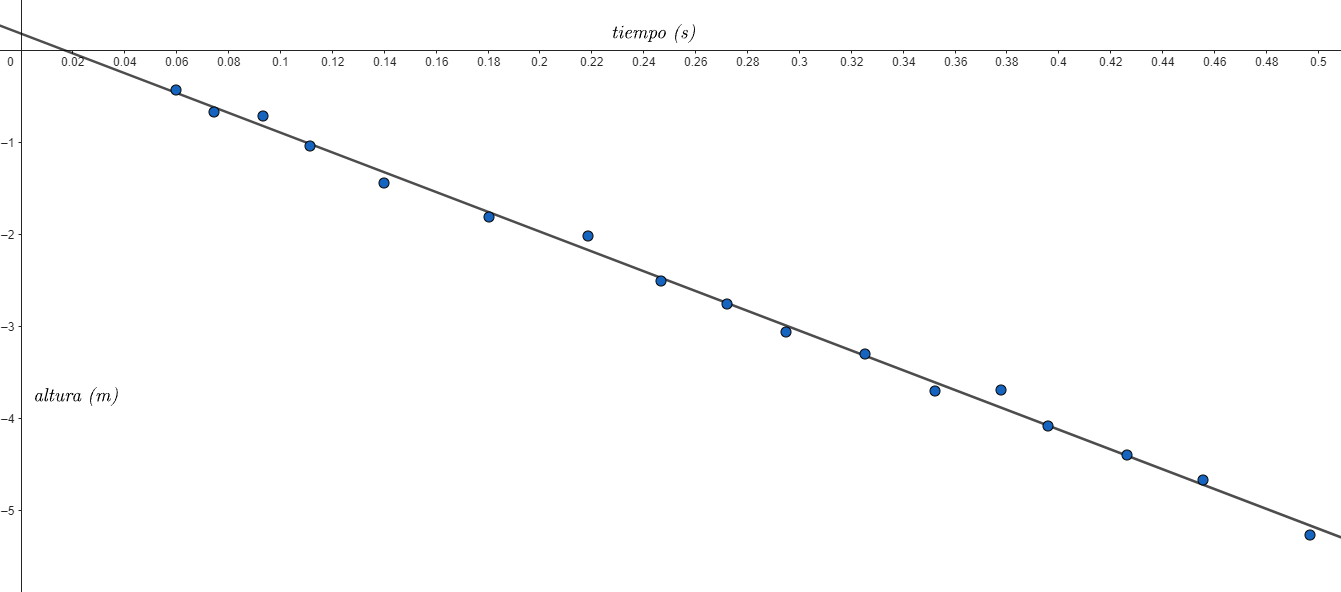
\includegraphics[width=1\linewidth]{vt2.png}
    \caption{Velocidad vs Tiempo (pelota 2)}
    \label{fig:enter-label}
\end{figure}

\begin{figure}[h]
    \centering
    
\includegraphics[width=1\linewidth]{image2.png}
    \caption{Posición en $y$ vs Tiempo (pelota 2)}
    \label{fig:enter-label}
\end{figure}



\section{DISCUSIÓN}
El experimento de caída libre realizado permitió obtener datos que reflejan el comportamiento de diversos objetos al ser soltados desde una altura de 2 metros. Los resultados obtenidos se analizaron mediante el software de video, permitiendo una precisión adecuada en la medición de los tiempos de caída. A continuación, se presenta un análisis de los resultados obtenidos, haciendo referencia a las gráficas de desplazamiento en función del tiempo ($y$ vs $t$) y de velocidad en función del tiempo ($v$ vs $t$). En la gráfica $y$ vs $t$, se observa que todos los objetos siguen una trayectoria característica del movimiento uniformemente acelerado. Esta trayectoria parabolica concuerda con la teoría del movimiento bajo la influencia de una aceleración constante, en este caso, la aceleración debida a la gravedad, se puso en comparación con la función $-gt^2$ para observar qué tan disperso está respecto al dato esperado. La pendiente de la gráfica de velocidad en función del tiempo $v$ vs $t$ proporciona una estimación directa de la aceleración gravitacional.
La gráfica $v$ vs $t$ muestra una relación lineal, lo cual es esperado para un objeto en caída libre en un campo gravitacional constante. \\

La pendiente de esta gráfica, al ser no altamente variable (sujeto a pequeños factores del entorno que podrían afectar la trayectoria), indica que la aceleración durante la caída se mantuvo aproximadamente constante. Este comportamiento lineal es consistente con las predicciones teóricas y confirma que la aceleración debida a la gravedad actúa de manera uniforme sobre los objetos.\\

A pesar de las medidas tomadas para minimizar la resistencia del aire, algunos objetos, como los filtros de café apilados y el cono de agua, presentaron desviaciones respecto a la idealidad teórica. Estos objetos, debido a su forma y masa, experimentan una mayor resistencia del aire, lo cual es evidente en las gráficas, donde se observa una ligera disminución en la aceleración aparente. En contraste, las pelotas de distintas masas, al tener una forma más aerodinámica y mayor densidad, mostraron comportamientos más cercanos a la idealidad de la caída libre en ausencia de resistencia. \\

El análisis de los tiempos de caída, al compararlos con los valores teóricos calculados mediante la ecuación $g = \frac{2y}{t^2}$ permitió determinar la aceleración gravitacional, no solo esto, al realizar la regresión lineal para cada punto del recorrido a la gráfica Velocidad vs Tiempo hemos obtenido una pendiente de $m= -10.1013217 \approx -10.101$ que realizando el cálculo de incertidumbre por mínimos cuadrados obtuvimos que $g = -10.101 \pm 0.2834$. Las discrepancias observadas entre los valores experimentales y los teóricos se pueden atribuir a factores como la resistencia del aire y posibles errores sistemáticos en la medición del tiempo.\\


\section{CONCLUSIONES} 
El experimento permitió observar de manera detallada el comportamiento de diferentes objetos en caída libre, confirmando en gran medida las predicciones teóricas del movimiento uniformemente acelerado bajo la influencia de la gravedad. Las gráficas obtenidas y su análisis contribuyen a una mejor comprensión de los factores que afectan la caída libre en condiciones reales, resaltando la importancia de considerar la resistencia del aire y las características de los objetos en el análisis experimental. Finalmente nuestro resultado más contundente es la deducción de la constante gravitacional quién es $g = -10.101 \pm 0.2834$.


% you can choose not to have a title for an appendix
% if you want by leaving the argument blank
\section{ REFERENCIAS}
\begin{itemize}
\item Serway, R. A., Jewett, J. W. (2008). "Física para ciencias e ingeniería.".
\item Resnick-Halliday. "Física Vol. 2, 5$^{ta}$ Edición, Editorial CECSA, México, 2005".
\item Aranzeta, C. G. (1986). "Introducción a la metodología experimental."
\item Oda-Noda, B. (2005). "Introducción al análisis gráfico de datos experimentales." 
\end{itemize}
% use section* for acknowledgment







\end{document}